\section{Integración}
\label{sec:integracion}

Para la integración de OpenL Tablets con {\SIDOSPU} existen dos alternativas.

La primera consiste en exponer las reglas por medio de un servicio web utilizando OpenL Rule Services. Esto nos permite integrar con distintas aplicaciones, sobre distintas plataformas, utilizar varias fuentes de datos y exponer varios proyectos y/o módulos mediante un único servicio web.

La segunda alternativa consiste en incluir OpenL Tablets como biblioteca y generar clases wrapper.
Estas últimas se generan en tiempo de ejecución a partir del contenido de las tablas en documentos Excel, exponiendo las reglas definidas en los mismos como métodos.
La principal ventaja de esta opción es que resulta en un menor costo de comunicación, dado que se realiza por medio de llamadas a métodos entre clases Java.

Considerando que las reglas serán utilizadas únicamente por {\SIDOSPU}, y estarán en un único proyecto, no pudiéndose sacar partido de los beneficios de un servicio web, se decidió utilizar la segunda opción.
%
%
El diagrama en la \cref{fig:integration} muestra un esquema de la integración resultante.
Los rectángulos representan una o varias clases Java, siendo la comunicación entre las mismas por llamado de sus respectivos métodos.

\begin{figure*}
    \centering
    \begin{tikzpicture}[
            auto,
            inner sep=3mm,
            box/.style={draw, rectangle, align=center},
            alt-box/.style={draw, rectangle, align=center, rounded corners=12pt},
            pre/.style={Stealth-},
            post/.style={-Stealth},
            alt-pre/.style={dashed, Stealth-},
            alt-post/.style={dashed, -Stealth},
        ]
        \node[box] (system) {SI-DOSPU};
        \node[box, right=of system] (service) {CalculoReglasServiceImpl}
        edge[pre] (system);
        \node[box, below=0.5cm of service] (clases) {Clases Integración}
        (clases.west) edge[post] (system);
        \node[box, right=of service] (wrapper)  {Clase Wrapper}
        edge[pre] (service)
        edge[post] (clases.east);
        \node[alt-box, above=of wrapper] (rules)  {Reglas (excel)}
        edge[alt-post] node {\small Compilado a} (wrapper)
        (rules.west) edge[alt-pre] node[swap] {\small Lee} (service);
    \end{tikzpicture}
    \caption{Integración OpenL Tablets con SI-DOSPU}
    \label{fig:integration}
\end{figure*}


\subsection{Clases de integración}\label{ssec:integracion:clases}

Como se mencionó en el \cref{sec:motores}, OpenL Tablets permite hacer uso directo de objetos Java dentro de las reglas.
Asimismo, permite hacer uso de clases de forma directa.
Sin embargo, las clases del {\SIDOSPU} lidian con cuestiones no del todo relevantes para el cálculo de las cuotas, como el manejo de errores y el acceso a datos que involucra comunicación con varias clases.
Para evitar contaminar con estos aspectos las reglas de cálculo, se crearon clase que los abstraen:
\begin{itemize}
    \item \scode{Afiliacion} encapsula complejidades de acceder a datos de la afiliación, como la categoría, subcategoría, si tiene cónyuge, etc.;
    \item \scode{Valores}, de manera similar, abstrae el acceso a otros valores del sistema relevantes pare el cálculo, como por ejemplo, el \acrshort{cmmu}; y
    \item \scode{Numero}, para poder operar sobre valores de tipo \scode{BigDecimal} utilizando operadores tales como +, -, *, /, etc.
\end{itemize}

\subsection{Cuota de Voluntario adherente}

% OpenL Tablets ofrece una variedad de tipos de tablas con distintas utilidades, en este trabajo se hizo uso de tablas de configuración, búsqueda y decisión. 
% La tabla de decisión posee la mayor flexibilidad y es la utilizada para la mayor parte de la lógica implementada. 

Esta sección sirve dos propósitos.
Por un lado describe como se especifica el cálculo de la cuota para voluntarios adherentes, y por otro lado introduce la sintaxis de las reglas.

OpenL Tablets ofrece una variedad de tipos de tablas \cite{openl-decision-table}.
Aquí describiremos brevemente el formato de las tablas de decisión, el cual es suficiente para expresar la lógica de negocio del cálculo de la cuota de afiliación.
%
La tabla de decisión en el \cref{tbl:cambio:original} aborda el caso de los voluntarios adherentes.
A continuación describimos su formato.

\begin{table*}[h]
    \centering
    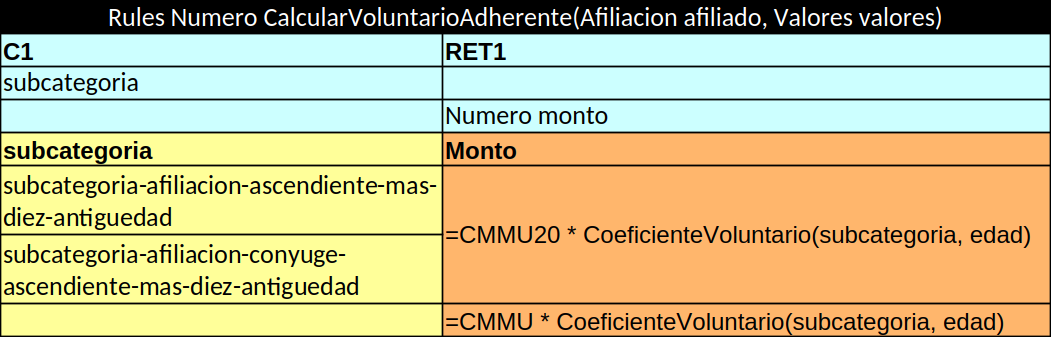
\includegraphics[width=1\textwidth]{voluntario.png}
    \caption{Cálculo de cuota de voluntario adherente}
    \label{tbl:cambio:original}
\end{table*}


% \begin{table*}[h]
%     \centering
%     \begin{tabular}{|p{7cm}|p{7cm}|}
%         \hline
%         \multicolumn{2}{|c|}{Rules Numero CalcularVoluntarioAdherente(Afiliacion afiliado, Valores valores)}                    \\ \hline
%         C1                                                              & RET1                                                \\ \hline
%         subcategoria                                                    &                                                     \\ \hline
%                                                                         & Numero monto                                        \\ \hline
%         subcategoria                                                    & Monto                                               \\ \hline
%         subcategoria-afiliacion-ascendiente-mas-diez-antiguedad         & =CMMU20 * CoeficienteVoluntario(subcategoria, edad) \\ \hline
%         subcategoria-afiliacion-conyuge-ascendiente-mas-diez-antiguedad &                                                     \\ \hline
%                                                                         & =CMMU * CoeficienteVoluntario(subcategoria, edad)   \\ \hline
%     \end{tabular}
%     \caption{Data from calcva.xls}
%     \label{tab:calcva}
% \end{table*}

% \begin{minted}{BNF}
% Rules <signatura>
% <signatura>::=<tipo> <nombre_tbl>(<pars>)
% <pars>::=<tipo> <nombre>
% \end{minted}


La fila 1 contiene el encabezado de la tabla.
En nuestro ejemplo: \tblcode{Rules} indica que la tabla contiene reglas,
\tblcode{Numero} es el tipo de retorno y \tblcode{CalcularVoluntarioAdherente(Afiliacion afiliado, Valores valores)} es el nombre de la tabla con sus dos parámetros.

La fila 2 define si la columna es una condición o valor de retorno, indicándose como  \tblcode{Cn} para la n-esima condición y \tblcode{RETn} para el n-esimo posible valor de retorno.
En el ejemplo, se indica que las columnas 1 y 2 corresponden a condiciones, y que en la 3 está el valor de retorno.

La fila 3 especifica la condición para cada columna en formato BEX \cite{openl-bex}.
Para \tblcode{C1} del ejemplo, se especifica \tblcode{subcategoria==valor}.
El lado izquierdo es inferido por nombre de uno de los atributos del parámetro \tblcode{afiliado} y el derecho se define en la fila 4.
La celda vacía para \tblcode{RET1} indica que no hay condiciones para ese retorno y se evalúa a \tblcode{Verdadero}.

% \begin{description}

    % \item[Fila 1: ] Contiene el encabezado de la tabla.
    %       En nuestro ejemplo: \tblcode{Rules} indica que la tabla contiene reglas,
    %       \tblcode{Numero} es el tipo de retorno y \tblcode{CalcularVoluntarioAdherente(Afiliacion afiliado, Valores valores)} es el nombre de la tabla con sus dos parámetros.

    % \item[Fila 2: ] Define si la/s columna/s es/son una condición o valor de retorno, indicándose como  \tblcode{Cn} para la n-esima condición y \tblcode{RET1} para el primer valor de retorno, respectivamente.
    %       En el ejemplo, se indica que las columnas 1 y 2 corresponden a condiciones, y que en la 3 está el valor de retorno.

    % \item[Fila 3: ] Especifica las condiciones para cada columna en formato BEX \cite{openl-bex}.
    %       Para \tblcode{C1} del ejemplo, se especifica \tblcode{subcategoria==valor}, donde el lado izquierdo es inferido por nombre de uno de los atributos del parámetro \tblcode{afiliado} y el derecho se define en la fila 4.
    %       La celda vacía para \tblcode{RET1} indica que no hay condiciones para ese retorno y se evalúa a \tblcode{Verdadero}.

    % \item[Fila 4: ] Define un parámetro por columna cuyos valores se definen a partir de la fila 6.
    %       Para \tblcode{C1} define de nombre \tblcode{valor} y tipo \tblcode{String}, y para \tblcode{RET1} el nombre \tblcode{monto} de tipo \tblcode{Numero}.

    % \item[Fila 5: ] Contiene nombres descriptivos para los parámetros, ignorados por el motor.

    % \item[Fila 6+:] Especifica los valores concretos para los parámetros.
    %       También pueden contener expresiones matemáticas o llamadas a otras reglas.

% \end{description}

La fila 4 define un parámetro por columna cuyos valores se definen a partir de la fila 6.
Para \tblcode{C1} define de nombre \tblcode{valor} y tipo \tblcode{String}, y para \tblcode{RET1} el nombre \tblcode{monto} de tipo \tblcode{Numero}.

La fila 5 contiene nombres descriptivos para los parámetros, ignorados por el motor.

Las filas 6, en adelante, especifican los valores concretos para los parámetros.
También pueden contener expresiones matemáticas o llamadas a otras reglas.
%
Para \tblcode{C1}, las filas 6 y 7 indican dos valores, que corresponden a ascendientes de primer grado con más de diez años de antigüedad y su cónyuge, respectivamente.
En ambos casos, el valor de \tblcode{RET1} es el mismo.
Se calcula como la multiplicación de un coeficiente, obtenido a partir de la tabla \tblcode{CoeficienteVoluntario} (no incluida en esta publicación), según la subcategoría y edad del afiliado, por el \acrshort{cmmu20}.
%
La fila 8 de \tblcode{C1} se encuentra vacía.
El motor interpreta que esta fila debe utilizarse por defecto para cualquier otro valor que no haya unificado aún.
El valor de retorno varía en este caso, ya que se utiliza el \acrshort{cmmu} en la multiplicación.

\subsection{Cuota de voluntario jubilado}

El cálculo del monto a abonar por jubilados es uno de los más complejos (junto con el caso de los voluntarios adherentes).
El mismo ocupa más de 150 líneas de código Java en la implementación original del \acrshort{si}.

Es cálculo inicia con el \cref{tbl:calculo:jubilado:1}.
Se debe notar un atajo utilizado en la notación para las expresiones de las dos condiciones, \tblcode{C1} y \tblcode{C2}.
Se coloca unicamente, el nombre del campo, que se obtiene del parámetro \tblcode{Afiliado}, cuando la expresión buscada es una igualdad con los valores que se colocaran en las celdas debajo.
Entonces, si el afiliado no tiene haber percibido actualizado, se retorna el valor calculado en el \cref{tbl:calculo:jubilado:sinhaber}. 
En caso de si tenerlo, el cálculo continua con el 
\cref{tbl:calculo:jubilado:conconyuge} o con el \cref{tbl:calculo:jubilado:sinconyuge}, dependiendo de si el afiliado tiene un cónyuge o conviviente que también sea titular en la obra social, o no.

\begin{table*}
    \centering
    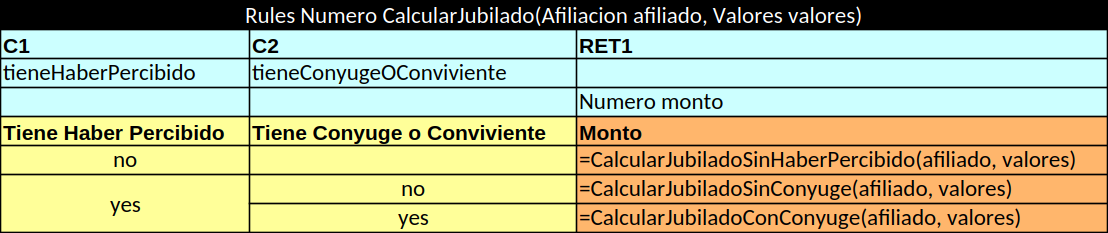
\includegraphics[width=.93\textwidth]{jubilado.png}
    \caption{Cálculo de cuota de jubilado}
    \label{tbl:calculo:jubilado:1}
\end{table*}

El cálculo del monto para un afiliado sin haber actualizado se muestra en el \cref{tbl:calculo:jubilado:sinhaber}.
Se toma como monto la cuota máxima de jubilado por un modificador, que depende de si el afiliado tiene un cónyuge o conviviente como afiliado familiar.

\begin{table*}
    \centering
    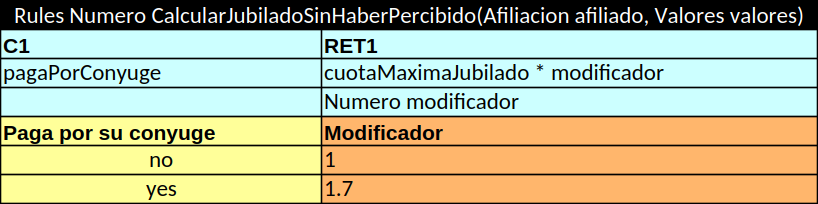
\includegraphics[width=0.7\textwidth]{jubiladoSinHaber.png}
    \caption{Cálculo de cuota de jubilado sin haber actualizado}
    \label{tbl:calculo:jubilado:sinhaber}
\end{table*}


\begin{table*}
    \centering
    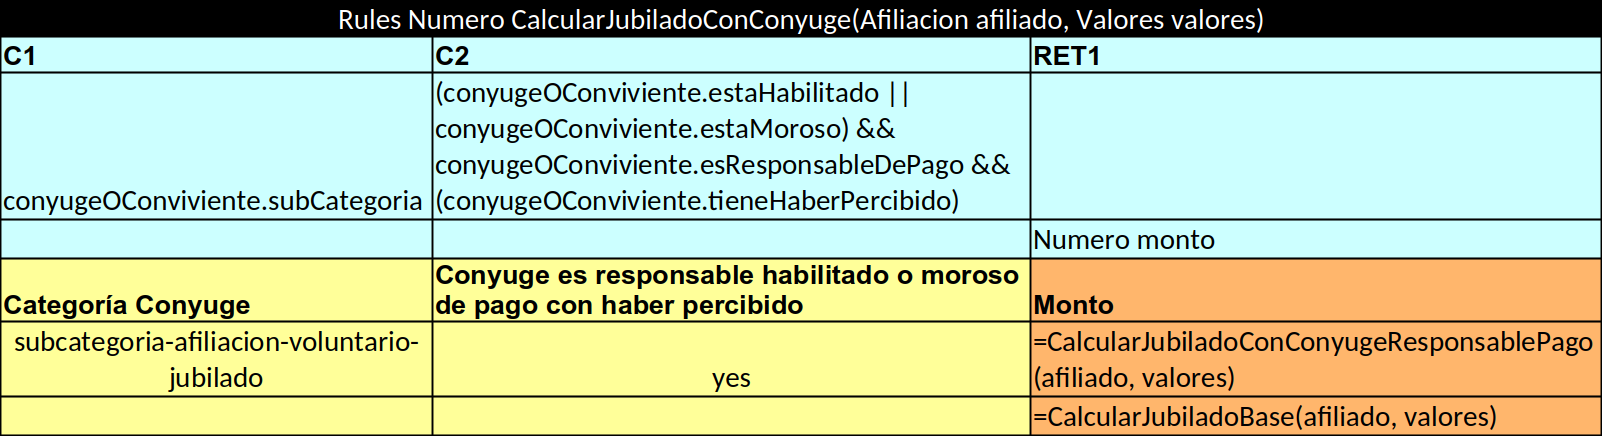
\includegraphics[width=1\textwidth]{jubiladoConConyuge.png}
    \caption{Cálculo de cuota de jubilado con cónyuge}
    \label{tbl:calculo:jubilado:conconyuge}
\end{table*}


\begin{table*}
    \centering
    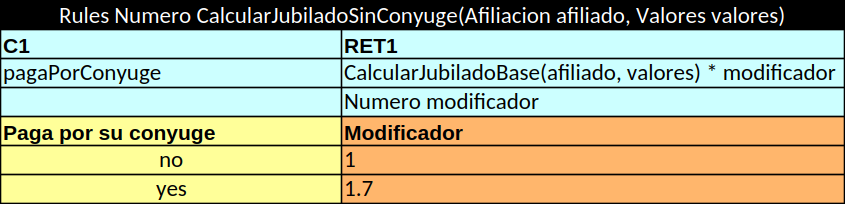
\includegraphics[width=0.7\textwidth]{jubiladoSinConyuge.png}
    \caption{Cálculo de cuota de jubilado sin cónyuge}
    \label{tbl:calculo:jubilado:sinconyuge}
\end{table*}


\begin{table*}
    \centering
    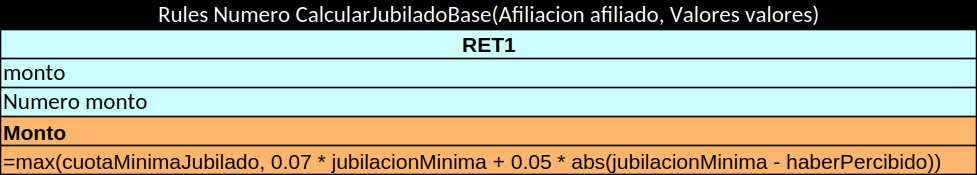
\includegraphics[width=0.8\textwidth]{jubiladoBase.png}
    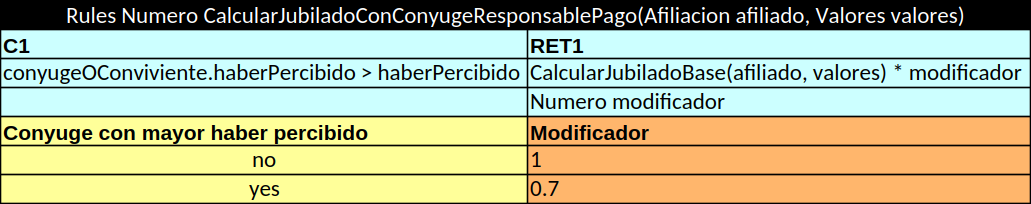
\includegraphics[width=0.8\textwidth]{jubiladoConConyugeResponsable.png}
    \caption{Cálculo cuota base jubilado}
    \label{tbl:calculo:jubilado}
\end{table*}

\subsection{Realizando un cambio}\label{ssec:integracion:cambio}
Para ilustrar las ventajas de estos cambios en el \SIDOSPU a la hora de realizar cambios en las reglas, consideremos la aplicación del siguiente cambio en el valor de las cuotas:

\emph{
    Para el cálculo de la cuota de un afiliado con categoría voluntario adherente y subcategoría agente \acrshort{unsl} con licencia, el monto de la cuota es equivalente al monto de los aportes y contribuciones 9\% del sueldo bruto que percibiría como si estuviera en actividad. De igual forma, dicho monto no puede ser inferior a los porcentajes de la \acrshort{cmmu} que se utilizan en el cálculo anteriormente presentado para la categoría y subcategoría.
}

Sin el uso del motor de reglas, este cambio implica el cambio/adición de una 32 líneas de código. Seguidamente, se debe volver a compilar y desplegar el sistema hacer estos cambios efectivos.

Por otra parte, haciendo uso del OpenL Tablets, con la integración descrite, se requiere realizar los cambios entre los cuadros \ref{tbl:cambio:original} y \ref{tbl:cambio:cambiado}. El cambio es detectado en tiempo de ejecución y se generan las nuevas clases wrapper, sin necesidad de volver a compilar o desplegar el sistema.



\begin{table*}
    \centering
    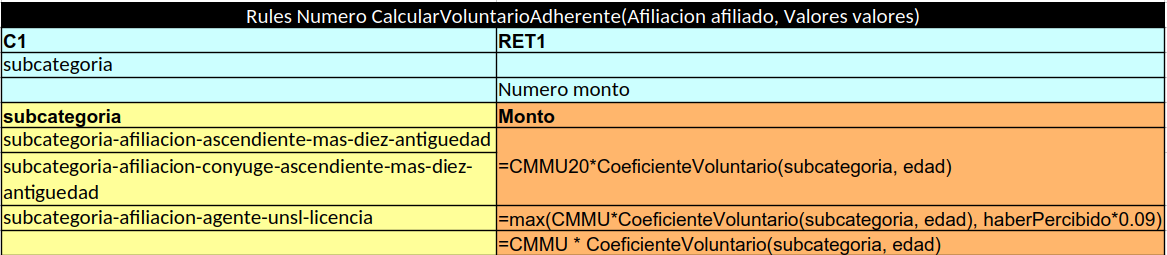
\includegraphics[width=0.8\textwidth]{voluntario_cambios.png}
    \caption{Cálculo modificado voluntario adherente modificado}
    \label{tbl:cambio:cambiado}
\end{table*}
